

\subsection{Kernel classifiers}



Trees simulated under different values of \gls{alpha} were visibly quite
distinct (\cref{fig:alphatrees}). In particular, higher values of \gls{alpha}
produce networks with a small number of highly connected nodes which, once
infected, are likely to transmit to many other nodes. This results in a more
unbalanced, ladder-like structure in the phylogeny, compared to networks with
lower \gls{alpha} values. None of the other three parameters produced trees
which were as easily distinguished from each other
(\cref{fig:Itrees,fig:mtrees,fig:Ntrees,fig:Itrees}).
Sackin's index, which measures tree imbalance, was significantly correlated with
all four parameters
    (for $\alpha$, $I$, $m$, and $N$ respectively: Spearman's rho =
     0.85,
     \ensuremath{-0.12},
     \ensuremath{-0.13},
     0.09;
     $p$-values
     $<10^{-5}$,
     $0.003$,
     $<10^{-5}$,
     $<10^{-5}$)
The ratio of internal to terminal branch lengths was negatively correlated with
\gls{alpha} and \gls{I}, and positively corelated with \gls{N} and \gls{m}
  (Spearman's rho
    \ensuremath{-0.84},
    \ensuremath{-0.69},
    0.1,
    0.18;
  $p$-values
    $0$,
    $2\!\times\!10^{-85}$,
    $4\!\times\!10^{-7}$,
    $0$).

\begin{figure}[ht]
  \centering
  \includegraphics{kernel-alpha-tree.pdf}
  \caption[Visibly distinctive trees simulated under three values of \gls{alpha}]{
    Epidemics simulated on \gls{BA} networks of 5000 nodes, with \gls{alpha}
    equal to 0.5, 1.0, or 1.5, until 1000 individuals were infected.
    Transmission trees were created by sampling 500 infected nodes. Higher
    \gls{alpha} values produced networks with a small number of
    highly-connected nodes, resulting in highly unbalanced, ladder-like trees.
  }
  \label{fig:alphatrees}
\end{figure}

\Cref{fig:kpca} shows \gls{kPCA} projections of the simulated trees onto the
first two principal components of the kernel matrix. The figure shows only the
simulations with 500-tip trees and, for all parameters except $I$, 1000
infected nodes. The three \gls{alpha} and \gls{I} values considered are well
separated from each other in feature space. On the other hand, the three
\gls{N} values overlap significantly, and the three \gls{m} values are
virtually indistinguishable. Similar observations can be made for other values
of \gls{I} and the number of tips
(\cref{fig:alphakpca,fig:Nkpca,fig:Ikpca,fig:mkpca}). The values of \gls{I} and
\gls{N} separate more clearly with larger numbers of tips, and in the case of
\gls{N} larger epidemic sizes.

\begin{figure}[ht]
  \centering
  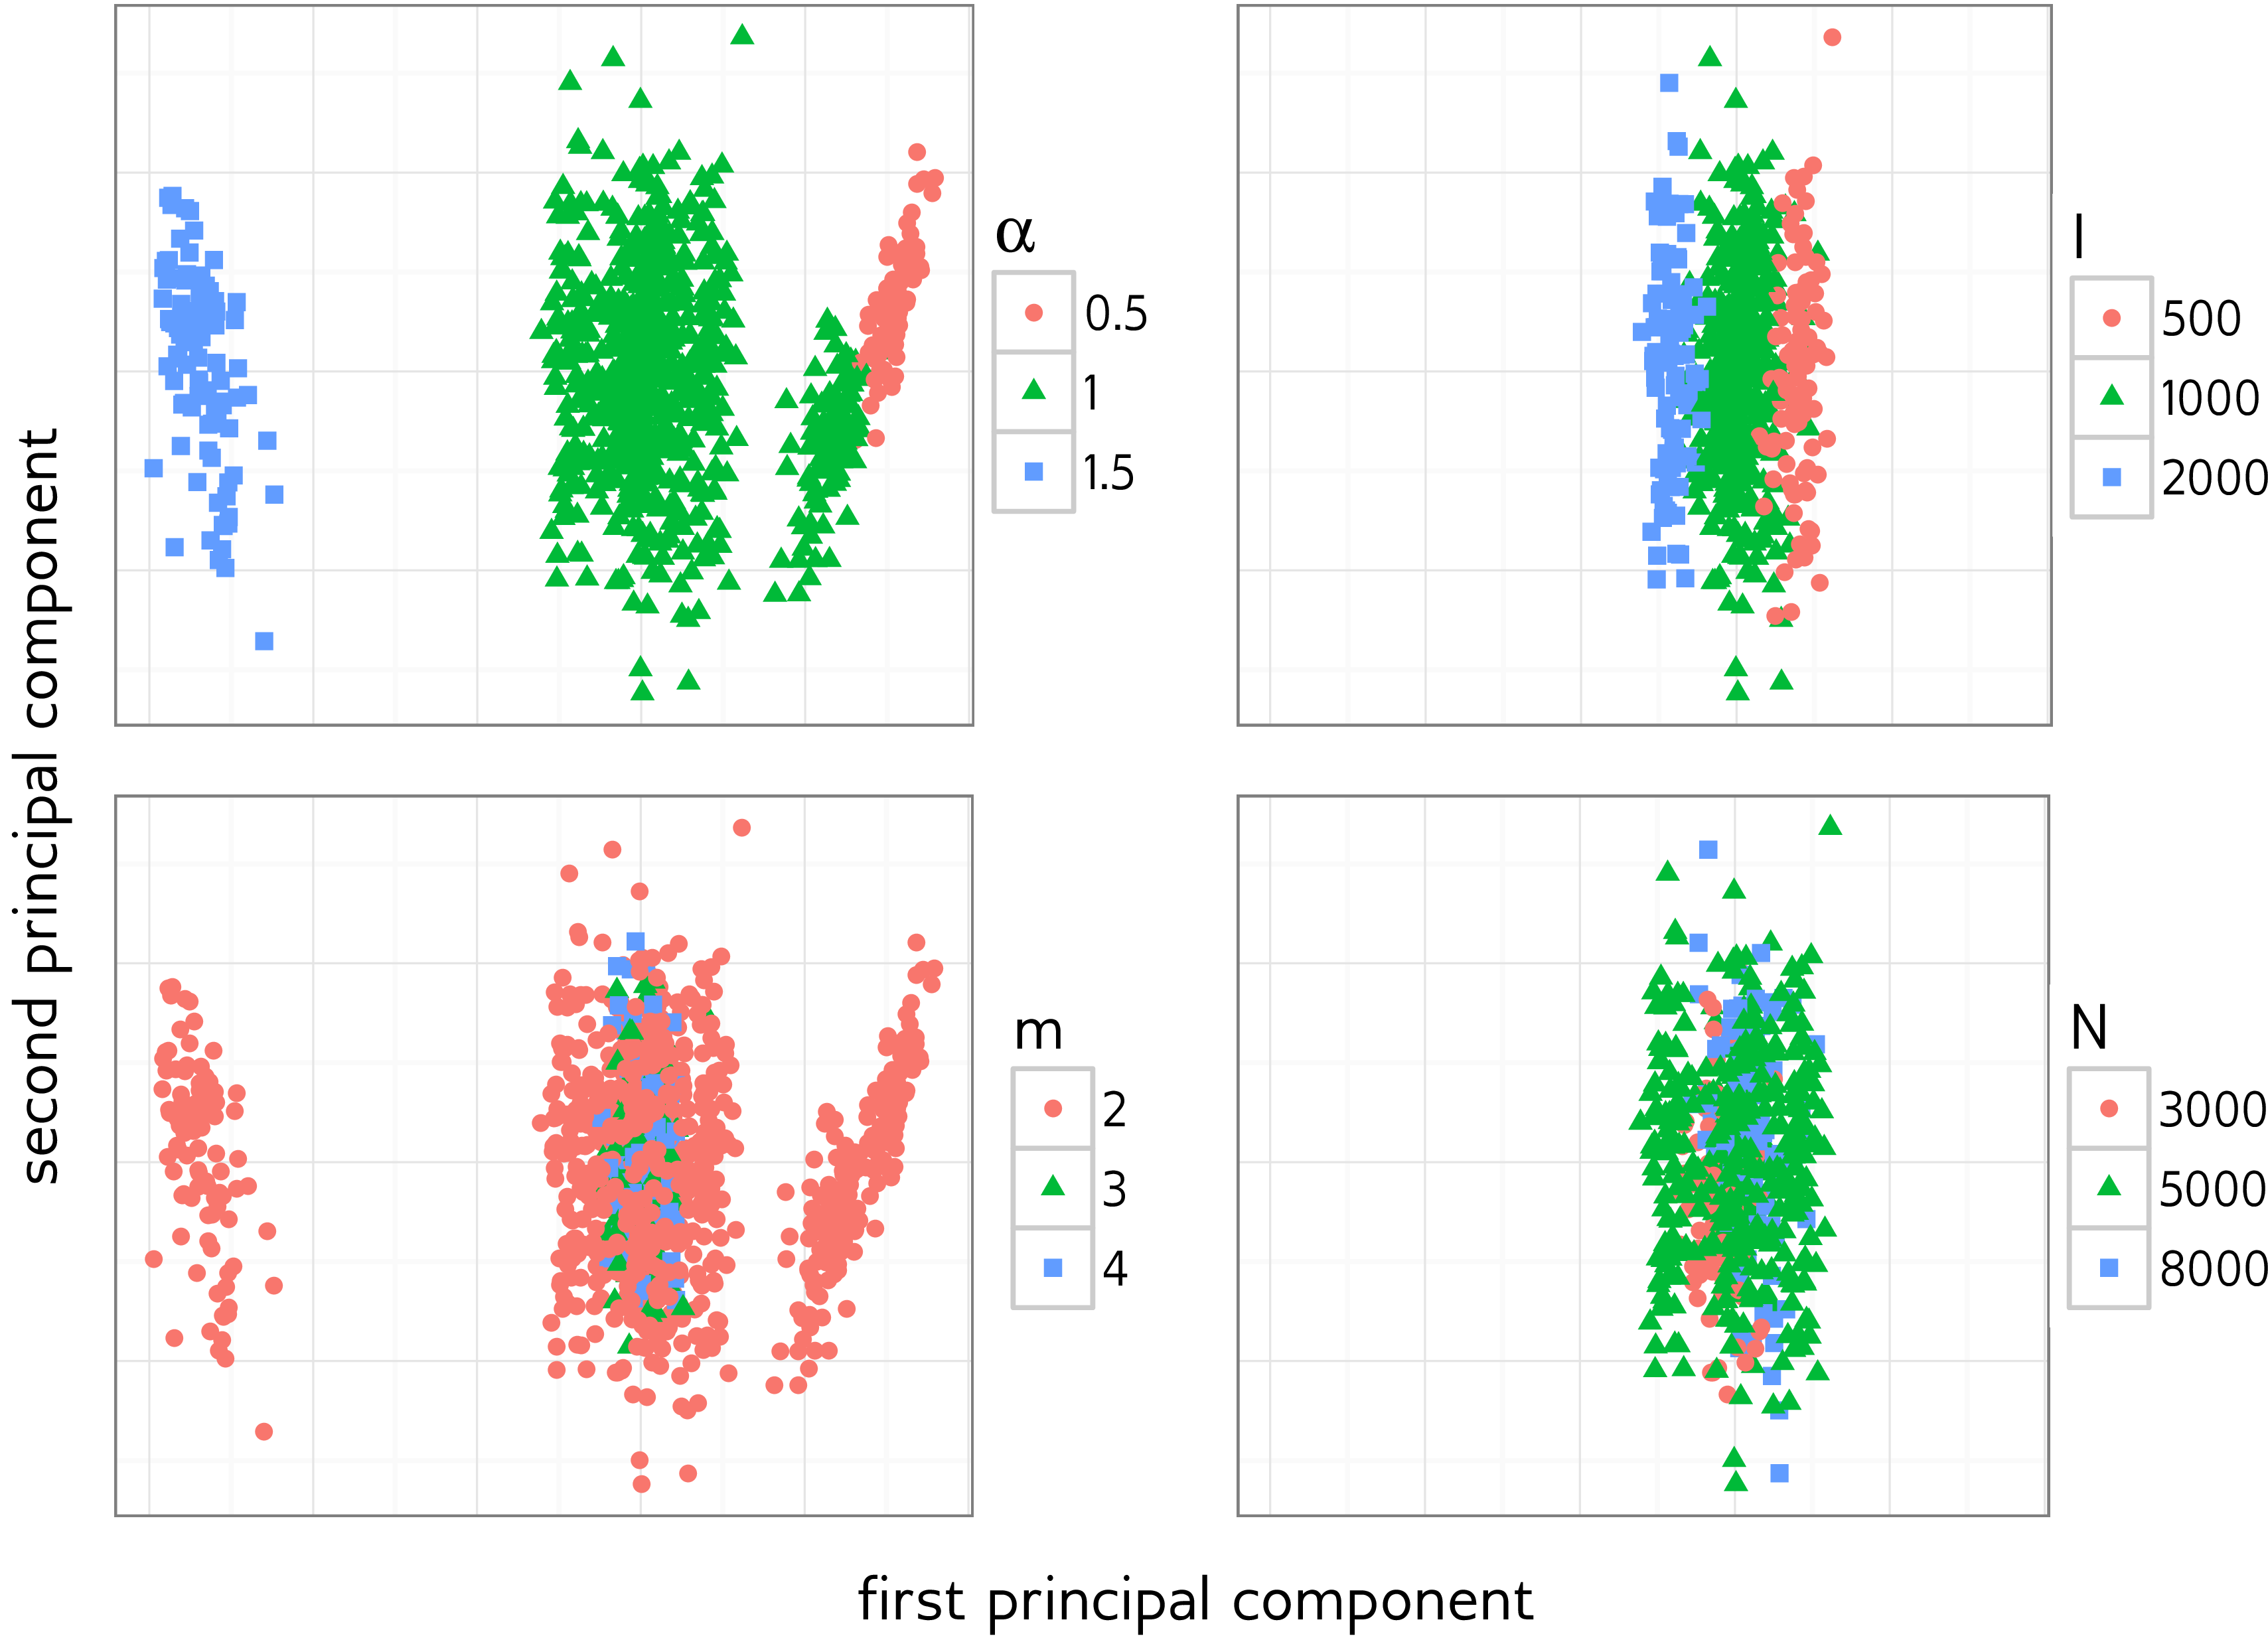
\includegraphics{kernel-kpca.pdf}
  \caption[\gls{kPCA} projections of simulated trees under varying \gls{BA}
           parameter values]{
    Each parameter of the \gls{BA} model was individually varied to produce 300
    simulated trees. Kernel matrices were formed from all pairwise kernel
    scores among each set of 300 trees. The trees were projected onto the first
    two principal components of the kernel matrix calculated using \gls{kPCA}.
    All trees had 500 tips. The parameters not being varied were set to
    \gls{alpha} = 1, \gls{I} = 1000, \gls{m} = 2, and \gls{N} = 5000. The tree
    kernel meta-parameters were $\lambda = 0.3$ and $\sigma = 4$.
  }
  \label{fig:kpca}
\end{figure}



Accuracy of the \gls{kSVM} classifiers varied based on the parameter being
tested (\cref{fig:rsquared}, left). Classifiers based on two other tree
statistics, the \gls{nltt} and Sackin's index, generally exhibited worse
performance than the tree kernel, although the magnitude of the disparity
varied between the parameters (\cref{fig:rsquared}, centre and right). The
results were largely robust to variations in the tree kernel meta-parameters
$\lambda$ and $\sigma$, although accuracy varied between different epidemic and
sampling scenarios
(\cref{fig:alphacrossv,fig:mcrossv,fig:Icrossv,fig:Ncrossv}).

When classifying $\alpha$, the kernel-SVM classifier had an average $R^2$ of 
    0.92,
compared to 
    0.56
for the \gls{nltt}-based SVM, and
    0.75
for the linear regression against Sackin's index. There was little variation
about the mean for different tree and epidemic sizes. No classifier could
accurately identify the $m$ parameter in any epidemic scenario, with average
$R^2$ values of 
  0.12 for \gls{kSVM},
  0.01 for the \gls{nltt}, and
  0.06
for Sackin's index. Again, there was little variation in accuracy between
epidemic scenarios, although the accuracy of the \gls{kSVM} was slightly higher
on 1000-tip trees.

The accuracy of classifiers $I$ varied significantly with the number of tips in
the tree. For 100-tip trees, the average $R^2$ values were
  0.7,
  0.55, and
  0.02
for the tree kernel, \gls{nltt}, and Sackin's index respectively. For 500-tip
trees, the values increased to
  0.93,
  0.83, and
  0.07.
Finally, the performance of classifiers for $N$ depended heavily on the
epidemic scenario. The $R^2$ of the \gls{kSVM} classifier ranged from
  0.08
for the smallest epidemic and smallest sample size, to
  0.82
for the largest. Likewise, $R^2$ for the \gls{nltt}-based SVM ranged from 
  0.01
to
  0.54.
Sackin's index did not accurately classify $N$ in any scenario, with an average
$R^2$ of
  0.03
and little variation between scenarios.

\begin{figure}[ht]
  \centering
  \includegraphics[width=\textwidth]{kernel-rsquared.pdf}
  \caption{
      Cross-validation accuracy of kernel-SVM classifier (left), SVM classifier
      using \gls{nltt} (centre), and linear regression using Sackin's index
      (right) for \gls{BA} model parameters. Kernel meta-parameters were set to
      $\lambda = 0.3$ and $\sigma = 4$. Each point was calculated based on 300
      simulated transmission trees over networks with three different values of
      the parameter being tested. Vertical lines are empirical 95\% confidence
      intervals based on 1000 two-fold cross-validations.
  }
  \label{fig:rsquared}
\end{figure}

\subsection{Grid search}




The accuracy of grid search estimates largely paralleled that of the \gls{kSVM}
classifiers. \Cref{fig:gridest} shows point estimates and 95\% highest density
intervals for each of the \gls{BA} parameters, for one replicate experiment
with 500-tip trees. For all parameters except $m$, the error of point estimates
was negatively correlated with the number of sampled tips in the tree (for
\gls{alpha}, \gls{I}, and \gls{N} respectively: Spearman's $\rho$ = 
    \ensuremath{-0.22},
    \ensuremath{-0.41},
    \ensuremath{-0.16};
$p$-value = 
    $4\!\times\!10^{-4}$,
    $2\!\times\!10^{-4}$,
    $0.01)$.
The highest density intervals obtained for all parameters were extremely wide,
occcupying $>$90\% of the grid in all cases. 

The \gls{alpha} parameter was the most accurately estimated, with point
estimates having an average deviation of 
    0.14
from the true value, on a grid from 0 to 2. The error was negatively correlated
with the true value of \gls{alpha} 
    (Spearman's $\rho$ = \ensuremath{-0.26},
     $p = 1\!\times\!10^{-5}$),
although the relationship was clearly nonlinear (\cref{fig:gridest,fig:gridalpha}).
The accuracy was highest for the test value \gls{alpha} = 1.25
    (mean error 0.02)
which exhibited markedly different behaviour than the other values in terms of
the distribution of kernel scores along the grid (\cref{fig:gridalpha}). In
particular, there was a very pronounced peak in scores around the true value,
in contrast to most other values where the scores were flat around the true
value. The peak was also observed to a lesser degree for \gls{alpha} = 1. The
average absolute error of the point estimates for \gls{I} was 
    298,
on a grid of 500 to 5000, and the errors were not significantly correlated with
the true value of \gls{I}. Kernel score distributions for all test values
exhibited the same rounded shape (\cref{fig:gridI}). 

For the other two parameters, \gls{m} and \gls{N}, accuracy was much poorer
(\cref{fig:gridest,fig:gridm,fig:gridN}). The average error for \gls{m} was
    1.31,
on a grid from 1 to 6; this error was positively correlated with increasing
\gls{m}
    (Spearman's $\rho$ = 0.25,
     $p = 6\!\times\!10^{-4}$).
This positive correlation was apparently due to the much lower error for $m =
1$ than for the other $m$ values (\cref{fig:gridm})
    (mean errors 0.1 for
     $m = 1$ vs. 1.5466667 for
     $m > 1$).
The value $m = 1$ causes the network to take on a distinct shape relative to
higher $m$ values, namely a tree (\textit{i.e.} there are no cycles,
\cref{subsec:treeshape}). The average error for \gls{N} was 
    2419,
on a grid from 1000 to 15000, and was positively correlated with the true value
of \gls{N}
    (Spearman's $\rho$ = 0.43,
     $p = 2\!\times\!10^{-12}$).

\begin{figure}[ht]
  \centering
  \includegraphics[width=\textwidth]{gridsearch-example}
  \caption[Grid search estimates of \gls{BA} model parameters]{Point estimates
      and 95\% highest density intervals for each \gls{BA} model parameter,
      obtained using grid search. Networks and transmission trees were
      simulated over a grid of values for each parameter while holding the
      others fixed. For a subset of the grid values ($x$-axis), test networks
      and trees were created and compared to each tree on the grid using the
      tree kernel. The kernel scores along the grid were normalized to resemble
      a probability distribution, from which the mode and highest density
      interval were calculated. Shown values correspond to one replicate
      experiment, with trees of size 500.
  } 
  \label{fig:gridest}
\end{figure}

\subsection{Accuracy of estimates with full ABC}



We used kernel-\gls{ABC} to estimate the parameters of the \gls{BA} model 
on simulated trees where the true parameter values were known. Point estimates
for each parameter are shown in Figure~\ref{fig:abcpt}. Of the four parameters,
\gls{alpha} was the most accurately estimated, with a median [IQR] absolute error
of 
    0.11 
    [0.05-0.18].
The accuracy of the estimates was not significantly different between values of
$m$ or $I$ (both one-way ANOVA,
    $p$ = 0.1
and 
    0.25),
although the errors when the true value of \gls{alpha} was zero were
significantly greater than the other values 
    (Wilcoxon rank-sum test, $p$ = \ensuremath{6.41\times 10^{-4}}).
The error in the estimated value of $I$ was
    306 
    [108-607].
Errors were significantly higher for $\alpha \geq 1$
    (Wilcoxon rank-sum test, $p$ = \ensuremath{6.12\times 10^{-4}})
and for $I$ = 2000
    ($p$ = \ensuremath{1.58\times 10^{-6}}),
but not for any values of $m$
    (one-way ANOVA, $p$ = 0.33).
The $m$ parameter was estimated correctly in
    37 \%
of simulations, with an error of one in
    40 \%
and of two or more in 
    22 \%
(the only possible $m$ values were 2, 3, 4, or 5). The true values of
$m$ and $I$ did not significantly affect the error
    (one-way ANOVA, $p$ = 0.5 and
                          0.68),
but the accuracy was significantly lower for integral than non-integral
values of \gls{alpha}
    (Wilcoxon rank-sum test, $p$ = \ensuremath{7.2\times 10^{-3}}).
Finally, the total number of nodes \gls{N} was consistently over-estimated by
about a factor of two
    (error \ensuremath{6.59\times 10^{3}} 
    [\ensuremath{4.21\times 10^{3}}-\ensuremath{8.28\times 10^{3}}]).
No other parameters influenced the accuracy of the $N$ estimates 
    (one-way ANOVA, $p \geq$ NA).

\Cref{fig:abcex} shows the \gls{ABC} approximation to the posterior
distribution on the \gls{BA} parameters for one simulation (equivalent plots
for all the simulations can be found in the supplemental materials). \Gls{HPD}
intervals around \gls{alpha} and \gls{I} were narrow relative to the region of
nonzero prior density, whereas the intervals for $m$ and \gls{N} were widely
dispersed. \Cref{tab:abchpd} shows point estimates and 95\% \gls{HPD}
intervals averaged over all simulations.

\begin{table}
    \centering
    % latex table generated in R 3.2.3 by xtable 1.8-2 package
% Fri Jun 17 12:51:45 2016
\begin{tabular}{lr>{\raggedleft\arraybackslash}p{2.5cm}>{\raggedleft\arraybackslash}p{2.5cm}>{\raggedleft\arraybackslash}p{2.5cm}}
  \hline
Parameter & True value & Mean point estimate & Mean HPD lower bound & Mean HPD upper bound \\ 
  \hline
$\alpha$ & 0.0 & 0.36 & 0.01 & 0.81 \\ 
   & 0.5 & 0.43 & 0.04 & 0.83 \\ 
   & 1.0 & 0.90 & 0.51 & 1.09 \\ 
   & 1.5 & 1.52 & 1.26 & 1.81 \\ 
  $I$ & 1000 & 1450 & 651 & 2592 \\ 
   & 2000 & 2622 & 1114 & 4080 \\ 
  $m$ & 2 & 2.96 & 2.00 & 5.00 \\ 
   & 3 & 3.04 & 2.04 & 4.96 \\ 
   & 4 & 3.17 & 1.88 & 5.00 \\ 
  $N$ & 5000 & 9041 & 2613 & 14659 \\ 
   \hline
\end{tabular}

    \caption{Average widths of 95\% confidence intervals for \gls{BA} model
    parameters estimated with kernel-\gls{ABC}.}
    \label{tab:glm}
\end{table}

\subsection{Characterization of power-law exponent in Barab\'asi-Albert networks}

\Cref{tab:glm} shows the estimated parameters for a log-link \gls{GLM} fitted
to the observed distribution of \gls{gamma} values. The coefficients are
interpretable as multiplicative effects.

\begin{table}
    \centering
    % latex table generated in R 3.2.3 by xtable 1.8-2 package
% Tue Mar 15 09:15:55 2016
\begin{tabular}{rrrl}
  \hline
 & exp(Estimate) & Standard error & P-value \\ 
  \hline
(Intercept) & 1.63 & $5.1 \times 10^{-3}$ & $<10^{-5}$ \\ 
  $\alpha$ & 1.77 & $4.4 \times 10^{-3}$ & $<10^{-5}$ \\ 
  $m$ & 1.03 & $1.0 \times 10^{-3}$ & $<10^{-5}$ \\ 
  $N$ & 1.00 & $5.8 \times 10^{-7}$ & $<10^{-5}$ \\ 
  $\alpha \times m$ & 1.00 & $8.7 \times 10^{-4}$ & $<10^{-5}$ \\ 
  $\alpha \times N$ & 1.00 & $5.0 \times 10^{-7}$ & $<10^{-5}$ \\ 
  $m \times N$ & 1.00 & $1.1 \times 10^{-7}$ & $<10^{-5}$ \\ 
  $\alpha \times m \times N$ & 1.00 & $9.9 \times 10^{-8}$ & $<10^{-5}$ \\ 
   \hline
\end{tabular}

    \caption{Estimated \gls{GLM} parameters for relationship between power-law
    exponent \gls{gamma} and \gls{BA} model parameters.}
    \label{tab:glm}
\end{table}

\subsection{Real data}



We applied kernel-ABC to five published HIV datasets (\cref{tab:data}),
and found substantial heterogeneity among the parameter estimates
(\cref{fig:abchpd}). Two of the datasets~\autocite{niculescu2015recent,
wang2015targeting} had estimated $\alpha$ values near unity (MAP estimates
[95\% HPD] 
  1.06 
  [0.63 - 
   1.27]
and
  1 
  [0.41 -
   1.16] respectively). 
Another two datasets~\autocite{li2015hiv, cuevas2009hiv} had lower estimated
values and wider HPD intervals
  (0.77 
  [0.01 - 
  1.03]
and
  0.66 
  [0.03 -
   0.84]). 
The \textcite{novitsky2014impact} data had an extremely low estimated $\alpha$
and a very wide HPD interval
  (0.17 
  [0.04 -
   1.39]). 
For all the datasets except \citeauthor{novitsky2014impact}, estimated values of
$I$ were below 2000, with narrow HPD intervals around two of the
datasets
  (\citeauthor{cuevas2009hiv}, 880 
  [290 -
   \ensuremath{1.51\times 10^{3}}];
   \citeauthor{niculescu2015recent}, 175
  [138 - 
   454])
and wider intervals around the other two
  (\citeauthor{li2015hiv}, \ensuremath{1.59\times 10^{3}} 
  [284 -
   \ensuremath{3.81\times 10^{3}}];
   \citeauthor{wang2015targeting}, 651
  [268 - 
   \ensuremath{4.24\times 10^{3}}]).
The \citeauthor{novitsky2014impact} data was again the outlier, with a very high
estimated $I$, and HPD interval spanning almost the entire prior region
  (\ensuremath{7.55\times 10^{3}} 
  [228 -
   \ensuremath{8.92\times 10^{3}}]).
No information was gleaned about the $m$ parameter, with the HPD interval
occupying the entire prior region for all datasets. The estimates of $N$ were
similarly uninformative, with the exception that the point estimate for the
\citeauthor{wang2015targeting} data was smaller
  (\ensuremath{5.84\times 10^{3}})
than the estimates for other datasets
 (average \ensuremath{8.93\times 10^{3}}).

\begin{figure*}[ht]
  \centering
  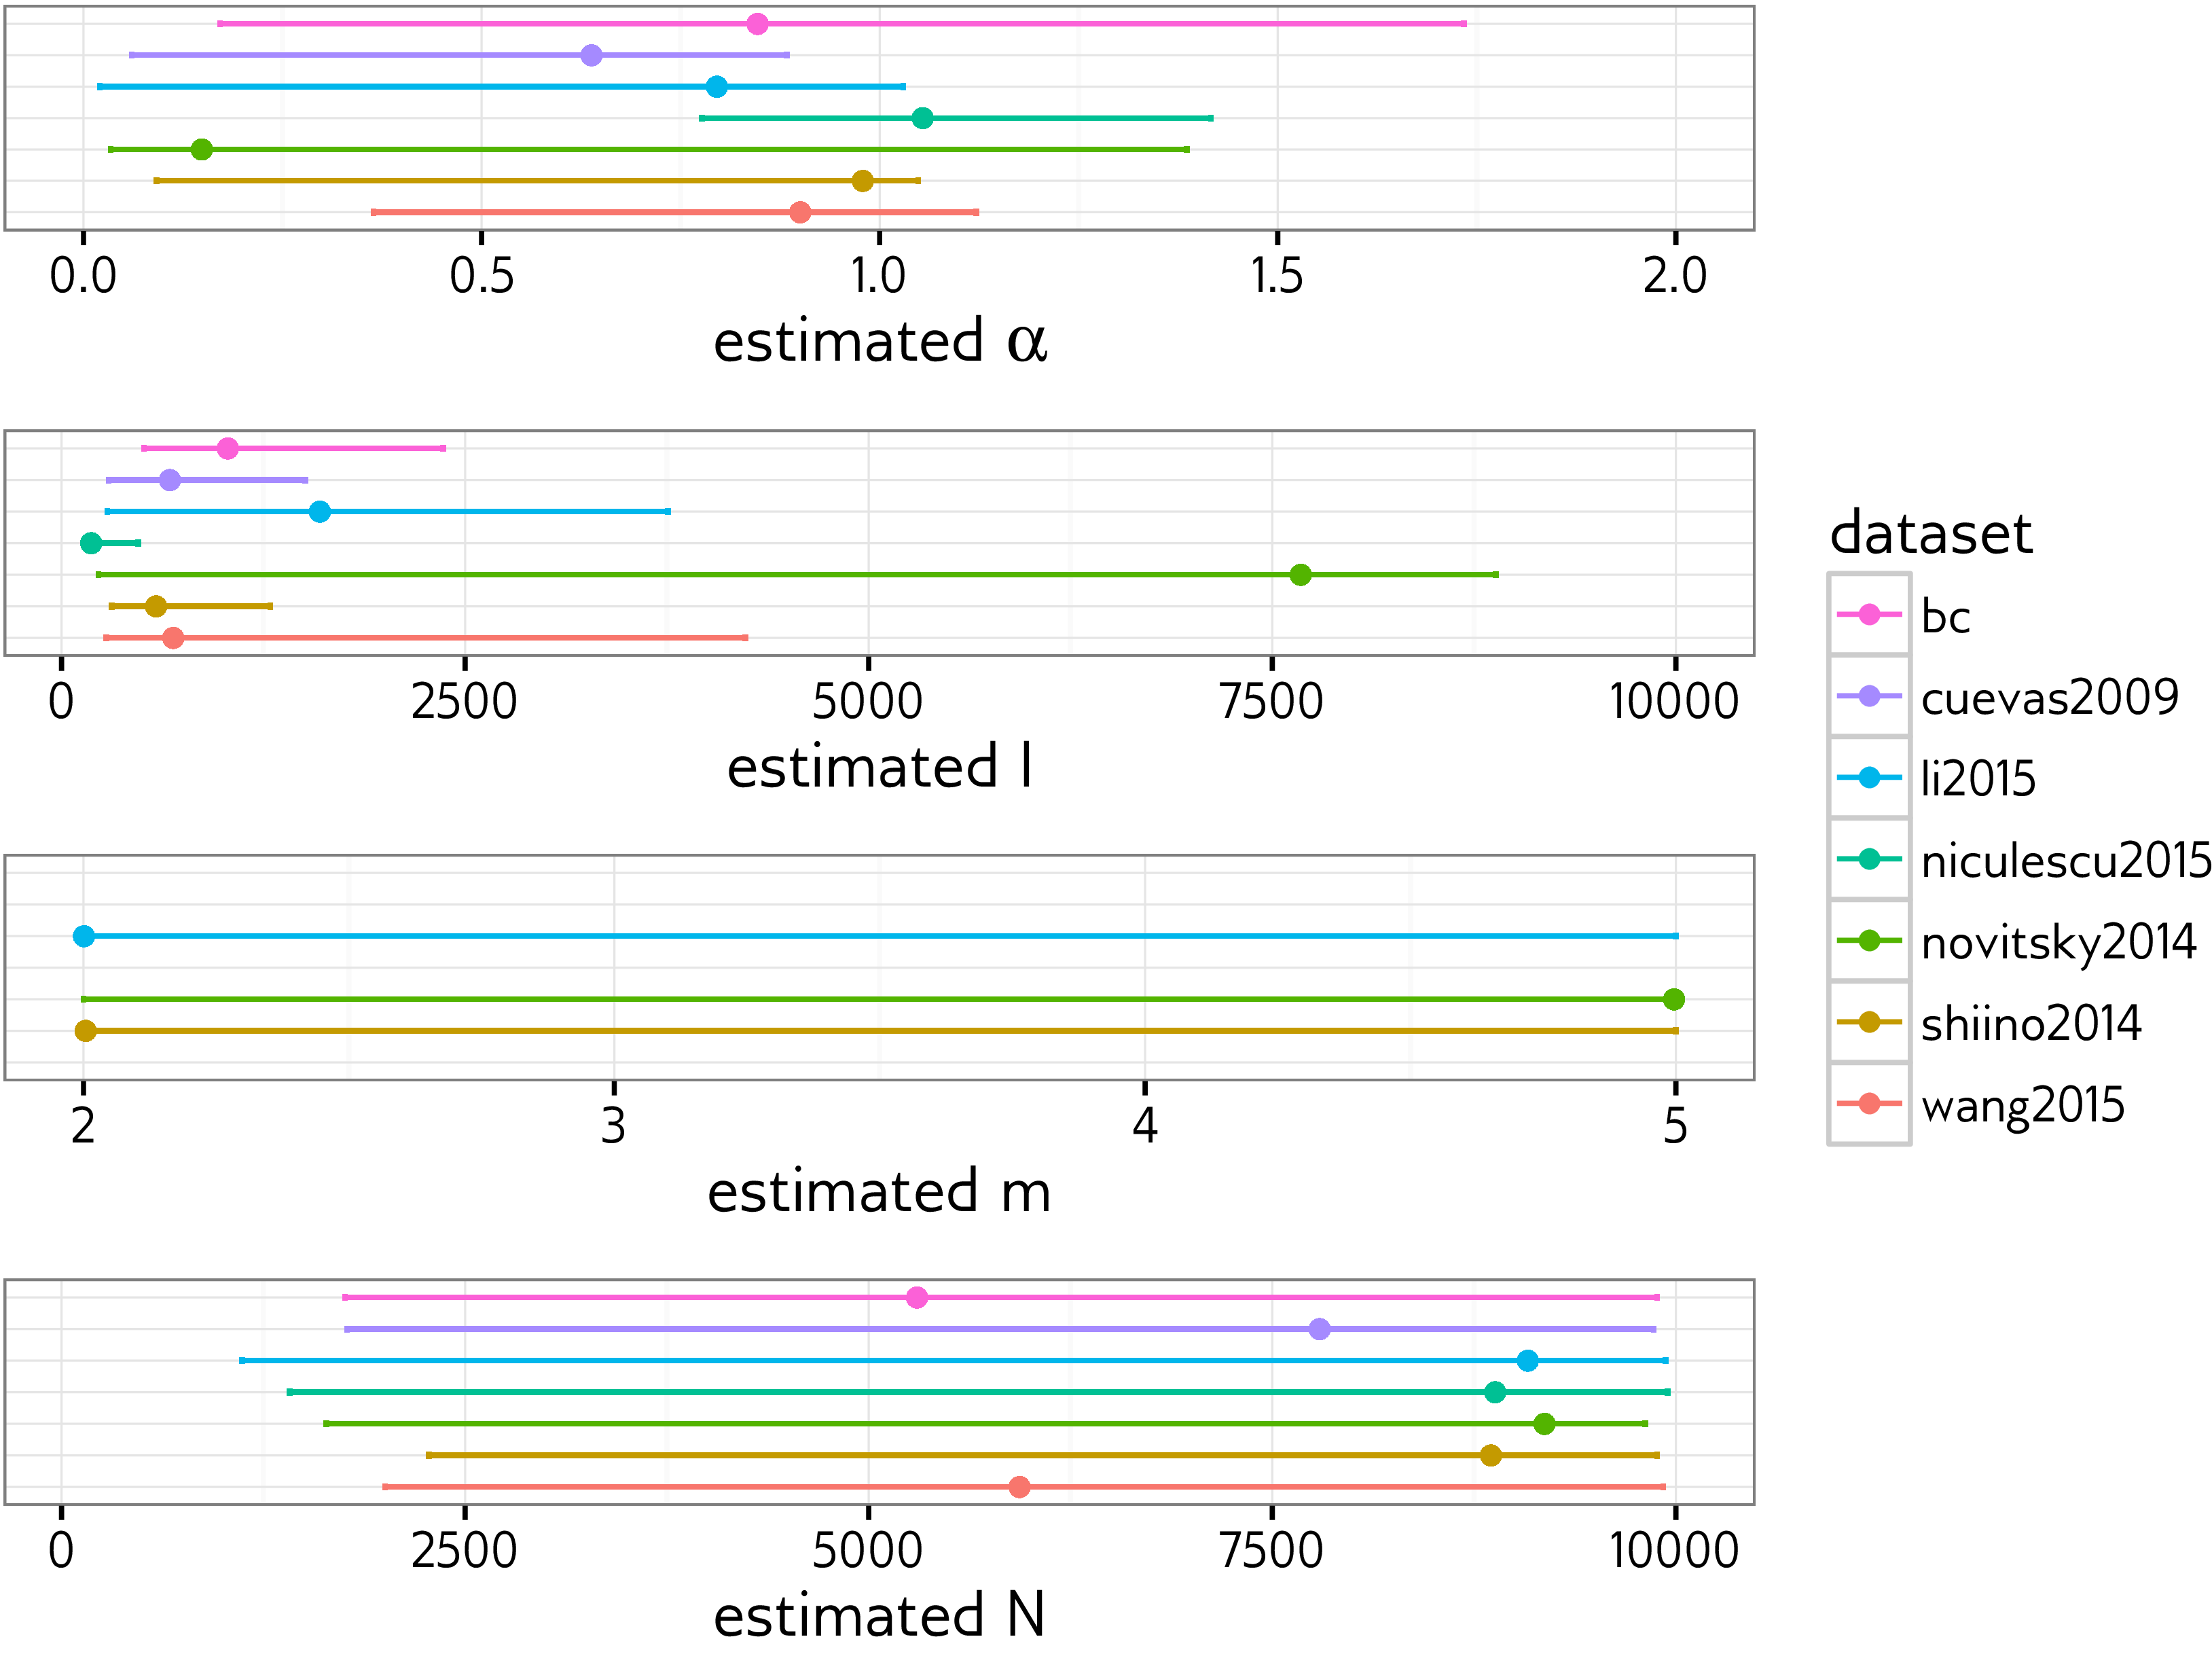
\includegraphics{realdata-hpd-bc.pdf}
  \vspace{8pt}
  \caption{
      Maximum \textit{a posteriori} point estimates and 95\% HPD intervals for
      parameters of the BA network model, fitted to five published HIV datasets
      with kernel-ABC.
  }
  \label{fig:abchpd}
\end{figure*}
